\chapter{Выполнения задания}

\section{Реализация алгоритма расчета TF для выборки документов}

В листинге \ref{lst:tf_alg} приведены реализации алгоритма выделения расчета термовой частоты для каждого терма из выборки документов. В качестве термов в данной реализации рассматриваются слова, состоящие из латинских букв. В качестве документов рассматриваются строки, состоящие из таких слов, пробелов и знаков пунктуации.

\clearpage

\lstinputlisting[label=lst:tf_alg,caption=Функция  реализации алгоритма расчета термовой частоты для каждого терма из выборки документов, firstline=1,lastline=30]{../tf_alg.c}

\section{Графовые представления}

\begin{figure}[h]
	\centering
	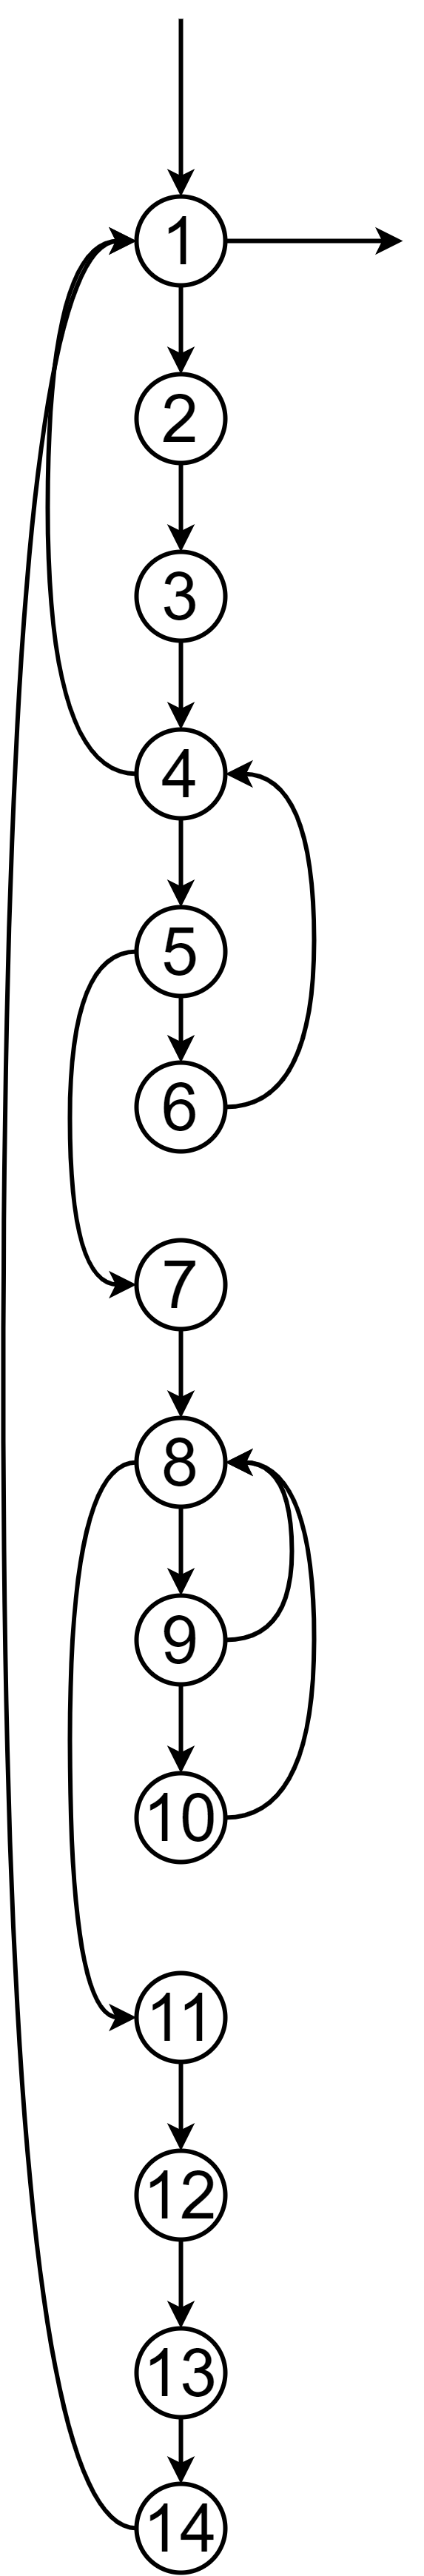
\includegraphics[height=0.9\textheight]{img/ГУ.png}
	\caption{Операционный граф}
	\label{fig:g1}
\end{figure}

\begin{figure}[h]
	\centering
	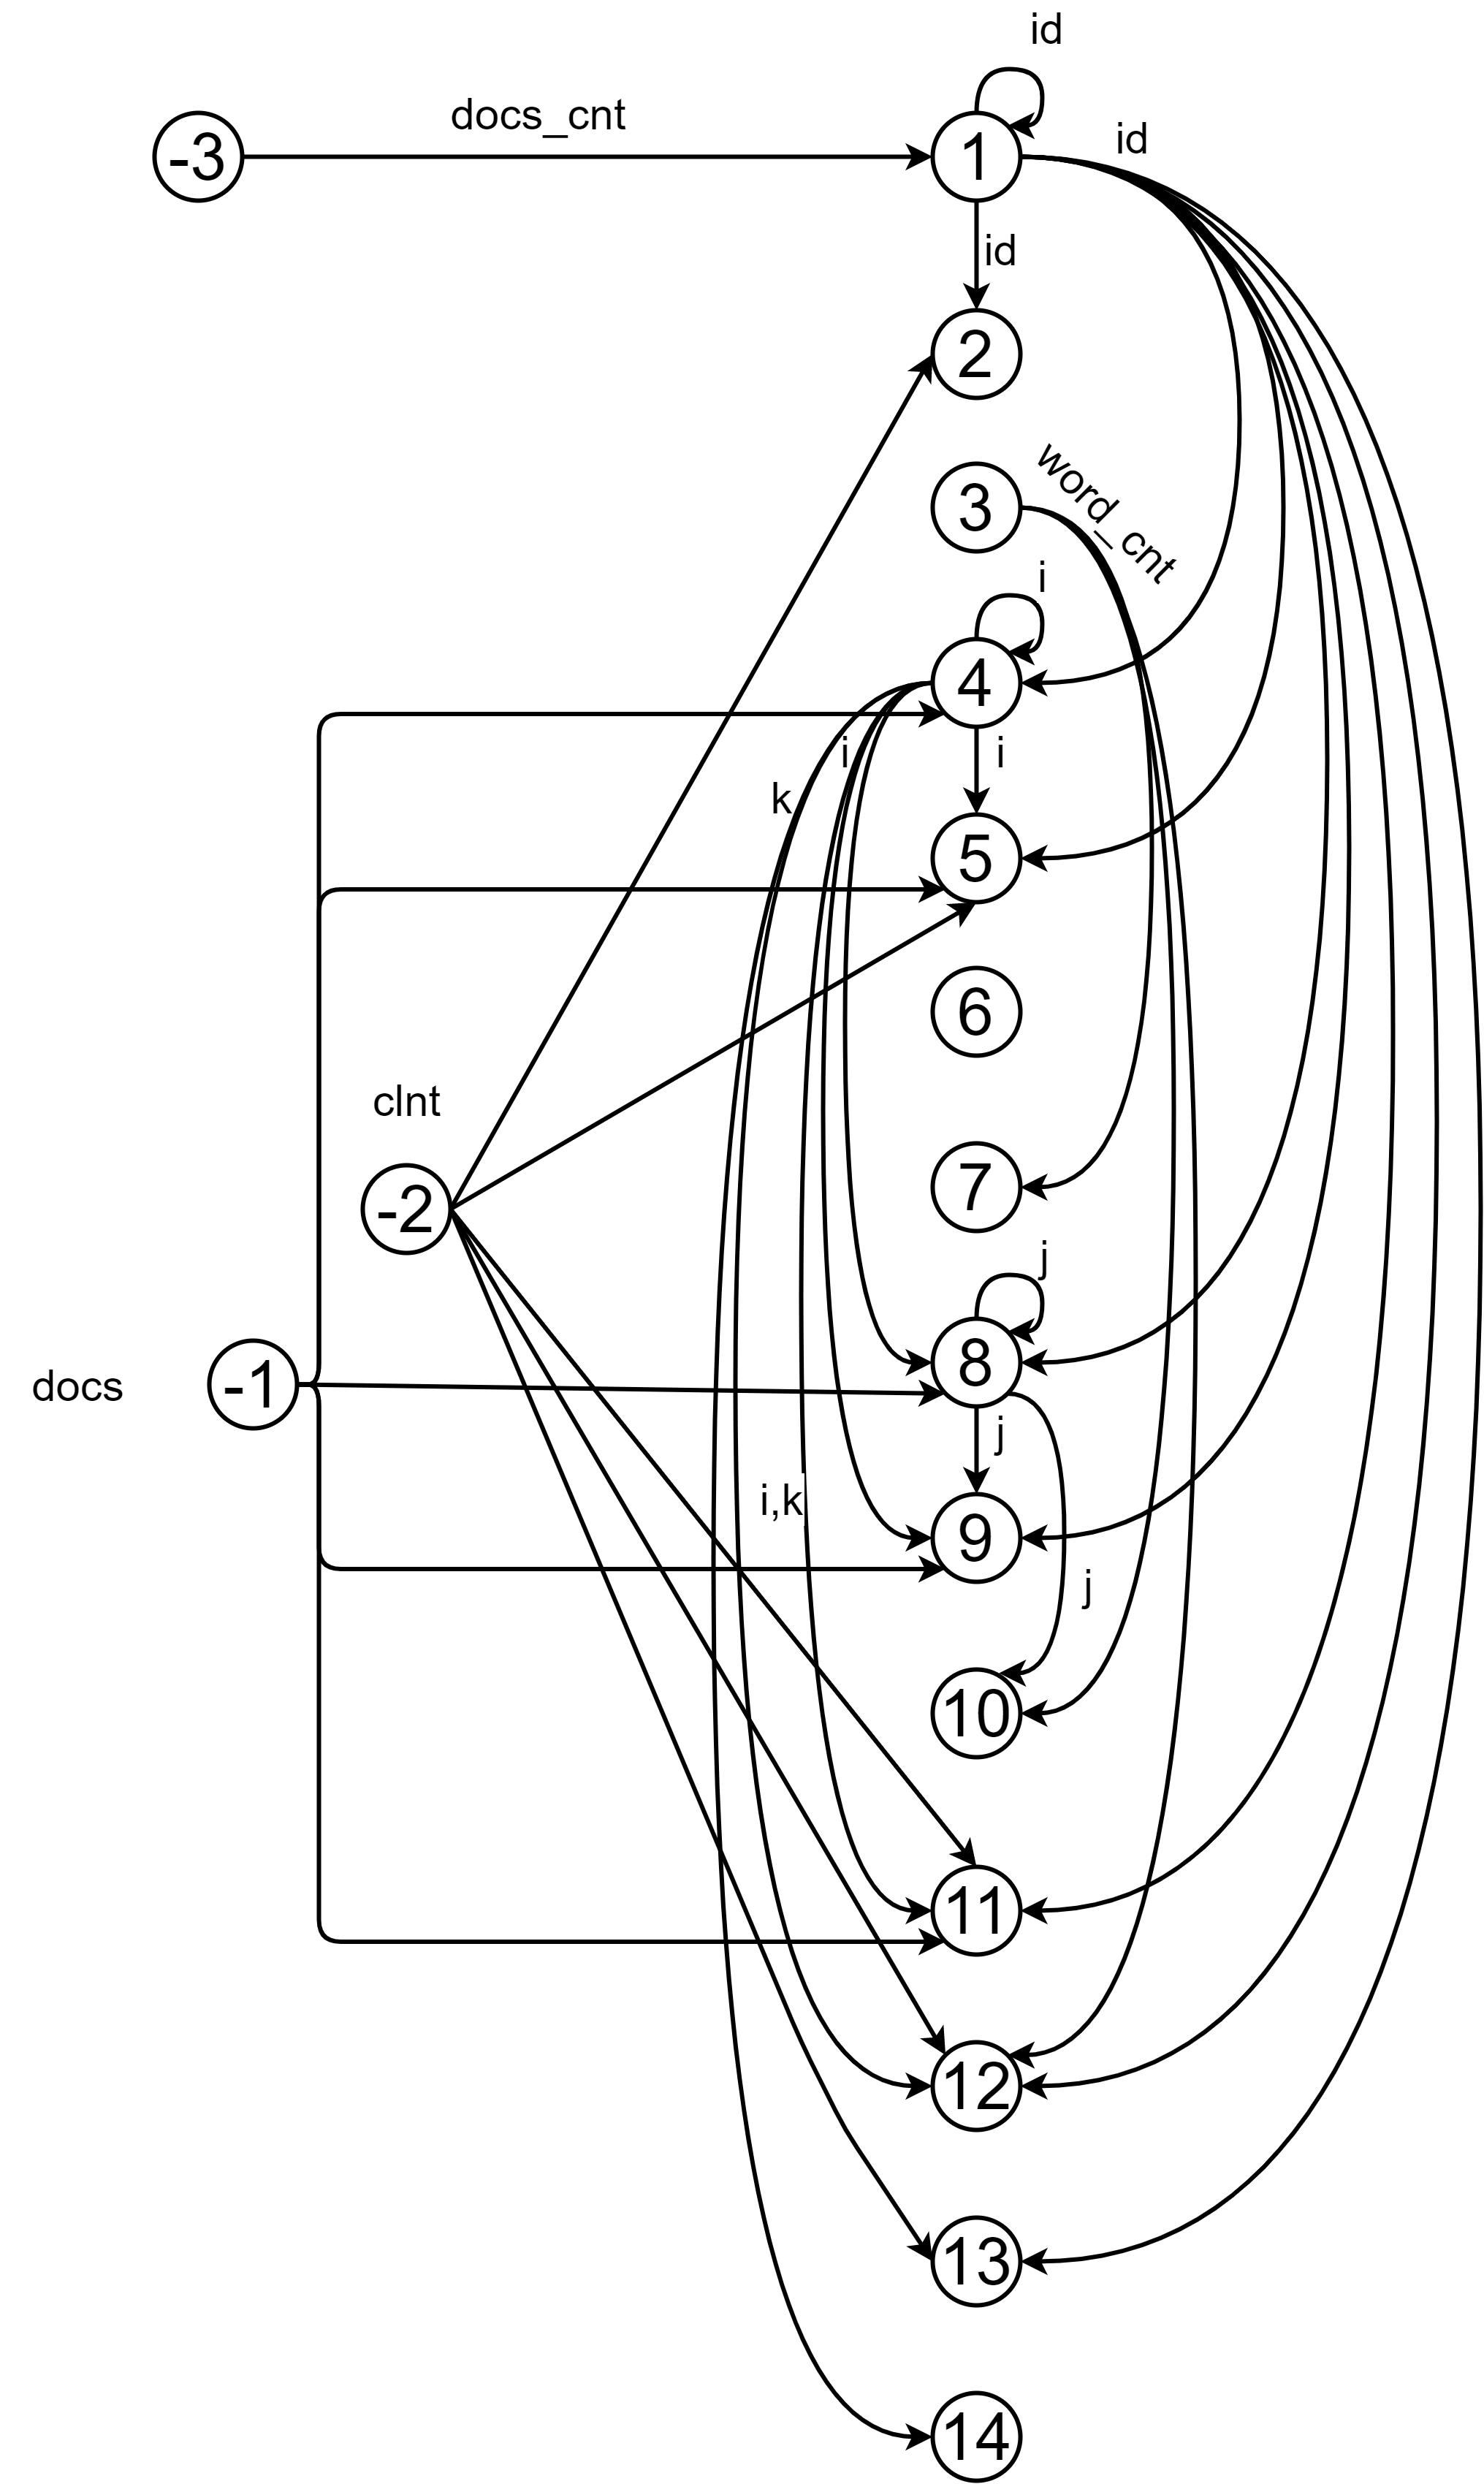
\includegraphics[height=0.9\textheight]{img/ИГ.png}
	\caption{Информационный граф}
	\label{fig:g2}
\end{figure}

\begin{figure}[h]
	\centering
	
\includegraphics[height=0.95\textheight]{img/ОИ.png}
	\caption{Операционная история}
	\label{fig:g3}
\end{figure}

\begin{figure}[h]
	\centering
	\includegraphics[height=0.95\textheight]{img/ИИ.png}
	\caption{Информационная история}
	\label{fig:g34}
\end{figure}

